\documentclass{cslthse-msc}
\usepackage[utf8]{inputenc}
\usepackage[english]{babel}
\usepackage{amsmath}
\usepackage{amsfonts}
\usepackage{amssymb}
\usepackage{amsthm}
%\usepackage{makeidx}
\usepackage{graphicx}
\usepackage[titletoc, header, page]{appendix}
\usepackage{hyperref}

\usepackage{float}
\usepackage{listings}

%\geometry{showframe}

\author{
	Anton Fagerberg \\
	{\normalsize \href{mailto:ada10afa@student.lu.se}{\texttt{ada10afa@student.lu.se}}}
}

\title{Work in progress title}
\subtitle{A {\LaTeX} class}
\company{Jayway}
\supervisor{Roger Henriksson, \href{mailto:Roger.Henriksson@cs.lth.se}{\texttt{Roger.Henriksson@cs.lth.se}}}
\examiner{Görel Hedin, \href{mailto:Gorel.Hedin@cs.lth.se}{\texttt{Gorel.Hedin@cs.lth.se}}}

\date{\today}
%\date{February 18, 2014}

\acknowledgements{
If you want to thank people, do it here, on a separate right-hand page. Both the U.S. \textit{acknowledgments} and the British \textit{acknowledgements} spellings are acceptable.

We would like to thank Lennart Andersson for his feedback on this template.
}

\theabstract{
This document describes the Master's Thesis format for the theses carried out at 
the Department of Computer Science, Lund University. 

Your abstract should capture, in English, the whole thesis with focus on the problem and solution in 150 words. It should be placed on a separate right-hand page, with an additional \textit{1cm} margin on both left and right. Avoid acronyms, footnotes, and references in the abstract if possible.

Leave a \textit{2cm} vertical space after the abstract and provide a few keywords relevant for your report. Use five to six words, of which at most two should be from the title.
}

\keywords{MSc, template, report, style, structure}

%% Only used to display font sizes
\makeatletter
\newcommand\thefontsize[1]{{#1 \f@size pt\par}}
\makeatother
%%%%%%%%%%


\begin{document}
\makefrontmatter

\chapter{Performance issues with HTTP 1.1}
Hypertext Transfer Protocol (HTTP) is an application protocol for distributed, collaborative, hypermedia information systems\cite{http-info}. The first standard version of HTTP 1.1 was released in January 1997\cite{rfc2068}. The next version, HTTP/2 (originally named HTTP 2.0), is expected to be released in 2015 (ändra här om det publiceras innan ex-jobbet är klart). Although HTTP/2 addresses several of the HTTP 1.1 performance issues, it is reasonable to assume that it will take many years before HTTP/2 fully replaces HTTP 1.1 as the protocol used on all web servers and even longer for many legacy systems and clients. It is therefore relevant to  acknowledge and mitigate the performance issues related to HTTP 1.1 even many years after the HTTP/2 release.

\section{Headers}

It is common in modern web applications to send a lot of HTTP requests toward a back-end API. These requests can be very small, such as an PUT request to update a single field but the actual payload can also be considered small when retrieving data from the server when it is compared to the total amount of data transmitted. Along with every HTTP request are typically plenty of headers. These headers can be a substantial part of every request and may therefore end up being the performance bottle neck if many small requests has to be transmitted.

As an example, consider the Instagram API\cite{instagram_api} which has an end-point where you can get information about a certain user account with a response serialised in JSON format. If a client was built which is supposed to show details about, for example, the 10 specific users. We can then benchmark how making 10 separate API requests would differ, in transmitted data size, from how it would behave if we could fetch all 10 users with one request.

\begin{figure}[H]
  \centering
    \begin{lstlisting}
{
    "data": {
        "id": "1574083",
        "username": "snoopdogg",
        "full_name": "Snoop Dogg",
        "profile_picture": "http://distillery...",
        "bio": "This is my bio",
        "website": "http://snoopdogg.com",
        "counts": {
            "media": 1320,
            "follows": 420,
            "followed_by": 3410
        }
    }
}
    \end{lstlisting}
  \caption{User data response from the Instagram API in JSON format.}
\end{figure}

HTTP requests can be benchmarked using cURL\cite{curl}. To make the requests authentic and look like it was made from an actual browser, we tell cURL to use the default headers provided by the browser Firefox. These headers includes among other things browsers the User-Agent, media types which are acceptable responses and so on. A local server running on port 9000 is used to simulate the the Instagram API.

\begin{figure}[H]
  \centering
\begin{lstlisting}[breaklines=true]
curl --trace-ascii - 'http://localhost:9000/user/snoopdogg' -H 'Host: localhost:9000' -H 'User-Agent: Mozilla/5.0 (Macintosh; Intel Mac OS X 10.10; rv:36.0) Gecko/20100101 Firefox/36.0' -H 'Accept: text/html,application/xhtml+xml,application/xml;q=0.9,*/*;q=0.8' -H 'Accept-Language: en-US,en;q=0.5' --compressed -H 'Connection: keep-alive' -H 'Pragma: no-cache' -H 'Cache-Control: no-cache'
\end{lstlisting}
  \caption{cURL command used in the benchmarks.}
\end{figure}

Performing this request will give us the following results:

\begin{figure}[H]
  \centering
\begin{lstlisting}[breaklines=true]
=> Send header, 355 bytes (0x163)
0000: GET /user/snoopdogg HTTP/1.1
001e: Accept-Encoding: deflate, gzip
003e: Host: localhost:9000
0054: User-Agent: Mozilla/5.0 (Macintosh; Intel Mac OS X 10.10; rv:36.
0094: 0) Gecko/20100101 Firefox/36.0
00b4: Accept: text/html,application/xhtml+xml,application/xml;q=0.9,*/
00f4: *;q=0.8
00fd: Accept-Language: en-US,en;q=0.5
011e: Connection: keep-alive
0136: Pragma: no-cache
0148: Cache-Control: no-cache
0161:
<= Recv header, 17 bytes (0x11)
0000: HTTP/1.1 200 OK
<= Recv header, 47 bytes (0x2f)
0000: Content-Type: application/json; charset=utf-8
<= Recv header, 21 bytes (0x15)
0000: Content-Length: 286
<= Recv header, 2 bytes (0x2)
0000:
<= Recv data, 286 bytes (0x11e)
\end{lstlisting}
  \caption{Results from cURL when sending an HTTP request to fetch one user. The actual response payload has been omitted.}
\end{figure}

We can from this information see that 355 bytes are sent as header data, 87 bytes are then received as header data (17 + 47 + 21 + 2) and the actual payload is 286 bytes. This means 61\% of every request to this user end-point are nothing but header data.

If we instead would expose an endpoint where all 10 users could be requested with one HTTP request which returned an array of JSON objects, we would get the following result:

\begin{figure}[H]
  \centering
\begin{lstlisting}[breaklines=true]
=> Send header, 446 bytes (0x1be)
0000: GET /users/snoopdog1,snoopdog2,snoopdog3,snoopdog4,snoopdog5,sno
0040: opdog6,snoopdog7,snoopdog8,snoopdog9,snoopdo10 HTTP/1.1
0079: Accept-Encoding: deflate, gzip
0099: Host: localhost:9000
00af: User-Agent: Mozilla/5.0 (Macintosh; Intel Mac OS X 10.10; rv:36.
00ef: 0) Gecko/20100101 Firefox/36.0
010f: Accept: text/html,application/xhtml+xml,application/xml;q=0.9,*/
014f: *;q=0.8
0158: Accept-Language: en-US,en;q=0.5
0179: Connection: keep-alive
0191: Pragma: no-cache
01a3: Cache-Control: no-cache
01bc:
<= Recv header, 17 bytes (0x11)
0000: HTTP/1.1 200 OK
<= Recv header, 47 bytes (0x2f)
0000: Content-Type: application/json; charset=utf-8
<= Recv header, 22 bytes (0x16)
0000: Content-Length: 2871
<= Recv header, 2 bytes (0x2)
0000:
<= Recv data, 2871 bytes (0xb37)
\end{lstlisting}
  \caption{Results from cURL when performing a HTTP request to fetch 10 users. The actual payload has been omitted.}
\end{figure}

From the results, we can see that the size of the sent headers has increased from 355 to 446 bytes because of the longer URL which specifies all users to fetch. The received headers are increased with just one byte from 87 to 88 because of the increased \emph{Content-Length} field. This results in a total header size of 534 bytes. The actual payload has increased from 286 bytes to 2871 bytes - about 10 fold which is expected since we request 10 users at once instead of one at a time. A very small increase in data is added because of the array-characters in the JSON format. By avoiding doing 10 separate requests and instead do one concatenated request, the overhead added because of all the headers have now been reduced from 61\% to 16\%. This number will scale with to the number of requests concatenated - the more requests concatenated, the lesser amount of overhead from HTTP headers.

\begin{figure}[H]
  \centering
    \begin{center}
      \begin{tabular}{ r | c | c }
        \textbf{\#} & \textbf{10 users, 10 request} & \textbf{10 users, 1 request} \\ \hline
        Headers & 4,420 B & 534 B \\ \hline
        Payload & 2,860 B & 2,871 B \\ \hline
        \% headers of total data & 61\% & 16\% \\ \hline
      \end{tabular}
    \end{center}
  \caption{Header and payload ratio when doing 10 separate or one concatenated request to fetch users.}
\end{figure}

The data displayed in this example should be viewed as a lower bound. In practise, HTTP cookies which are used for personalisation, analytics and session management are also sent with every HTTP request as headers and can add up to multiple kilobytes of protocol overhead for every single HTTP request\cite[p. 200]{HPBN}.

This is one of the issues that may (ändra "may" om det stämmer när http2 släpps) be mitigated by using HTTP/2 which remembers which headers that has already been sent and therefore doesn't need to retransmit them on subsequent requests\cite[p. 222]{HPBN}.

\section{Maximum TCP connections}
The HTTP 1.X protocol doesn't allow data to be multiplexed over the same connection\cite[p.194]{HPBN}. For this reason, browser vendors has introduced a connection pool of ~6 TCP connections per host (the HTTP 1.1 specification limits the pool to 2 connections\cite{rfc2616} per host, but modern browsers has refused to conform to this standard in order to decrease the load times).

A common way to deal with the connection limit is to use domain sharding. Since the limit of six TCP connections are on a host name basis, it is possible to create multiple subdomains to avoid this limit. If the subdomains \{shard1, shard2, \ldots\}.example.com where created and pointed to the same server, more than six TCP connections can be used in parallel at the same time from that machine. This approach is not without downsides as every new host requires a new DNS lookup, a TCP three-Way handshake and a slow start from TCP which can have negative impact on the load times\cite[p. 199]{HPBN} - just the DNS lookup typically takes 20-120 ms\cite[p. 63]{HPWS}. Another problem with domain sharding is that the browser always opens six connections per shard even if not all of them are used. In addition, domain sharding can be a complicated manual process and it is hard to calculate how many shards to use for optimal performance. When Yahoo investigated this problem they reached to conclusion that you should, as a rule of thumb, use at least two, but no more than four domain shards\cite{yahoo-performance-4}.

As an example, we can benchmark downloading thumbnails for an image gallery. Suppose we want to download 60 thumbnails, encoded in base-64 format, and the connection we are using has a lot of bandwidth but suffers from high latency.

If all images were downloaded by using a single HTTP request per thumbnail, we can see that the six TCP connection limit will become a bottleneck.

\begin{figure}[H]
  \centering
    \begin{center}
      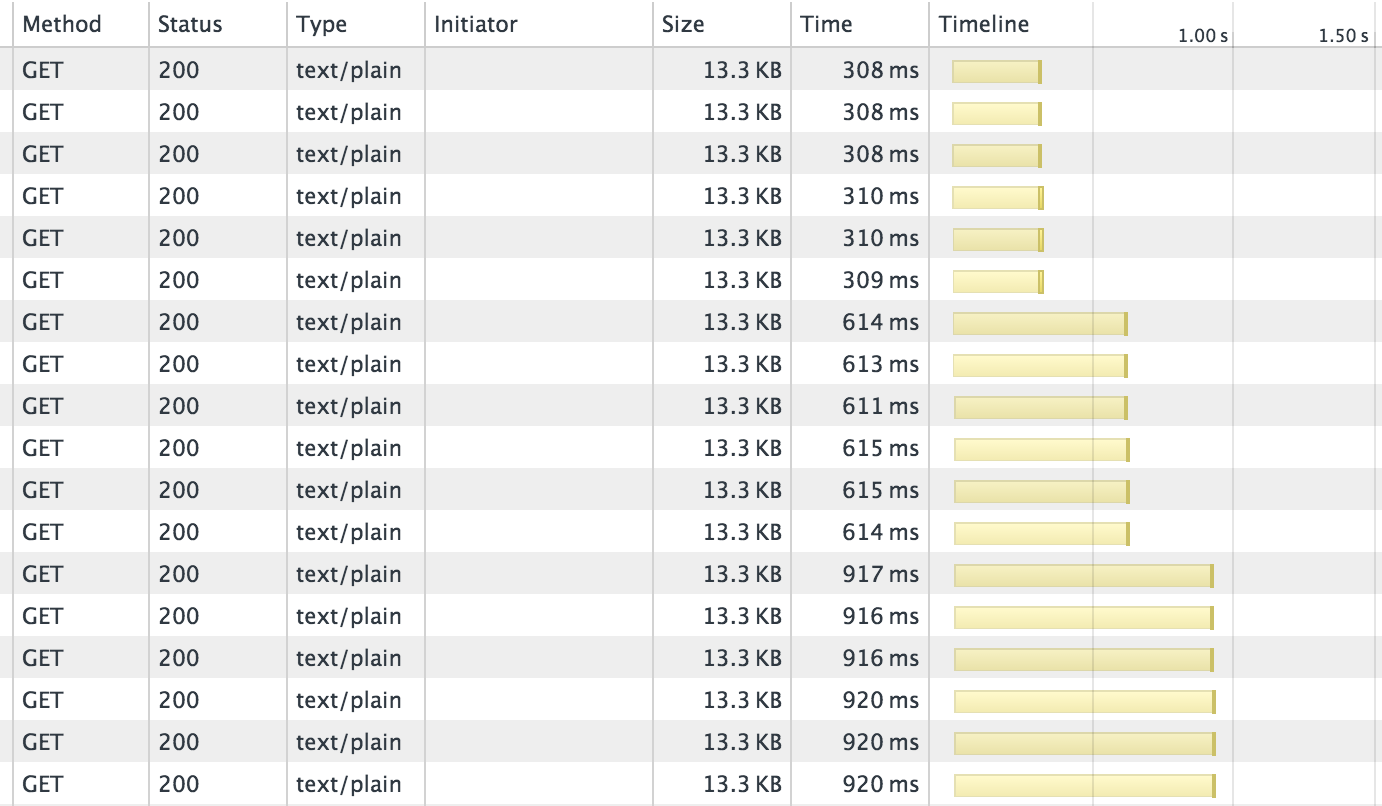
\includegraphics[width=0.9\textwidth]{images/chrome_latency_limit.png}
    \end{center}
  \caption{Chrome developer tools showing how the six TCP connection limit becomes a bottle neck on a connection with ~300 ms of latency.}
\end{figure}

We can calculate the total delay caused by latency in our example by this formula:

\begin{equation}
\mbox{total latency} = \mbox{number of thumbnails} * \frac{\mbox{latency per request}}{\mbox{number of parallel requests}}
\end{equation}

In our example, we fetch 60 thumbnails and with a latency of ~300 ms per request. Our browser can handle six parallel TCP connections which gives us the following result:

\begin{equation}
\mbox{total latency} = 60 * \frac{300}{6} = 3,000 \mbox{ ms}
\end{equation}

If we instead could concatenate these 60 thumbnail requests into one request and the response would contain all of the thumbnails - then we would only have to pay the latency cost once which would reduce the total latency by an order of magnitude from 3,000 ms to 300 ms.

It is worth pointing out that increasing the bandwidth would not resolve this problem as the latency is the only bottleneck in this scenario. It is not uncommon for browsers to wait idle for 100 - 150 ms before spending 5 ms to download an image which means that latency is accounting for 90-95\% of the total time for the HTTP requests\cite{latency}.

\subsection{Chunked responses}
When fetching thumbnails, you often want to display them as soon as each individual image has been loaded and not wait for the entire concatenated response. When using a concatenated request to fetch multiple resources at the same time, the server can use chunked transfer encoding in the HTTP response to send the thumbnail data in chunks\cite{chunked}. By doing so, images can be loaded as soon as they are available in the client, even if loaded out of order\cite{dropbox_chunked}.

\section{Compression}

All requested data should be compressed before it is sent to the client. A common compression algorithm used in HTTP requests is Gzip (GNU Zip) which works best on text-based files such as HTML, CSS and JavaScript. Gzip has an expected compression rate of 60-80\% when used on text-based files\cite[p. 237]{HPBN}.

It is worth mentioning that there are scenarios where Gzip compression applied to very small files can increase the total size because of the Gzip dictionary overhead. This problem can be mitigated by defining a minimum file size threshold\cite{google_gzip}.

As an example, arbitrary user data for 50 users was created and stored in JSON format. When this data was requested from the server without compression, the total content-length of the HTTP request payload amounted to 55,205 bytes. When applying Gzip compression to the same data, the content length was reduced to 16,563, which amounts to a space saving of 70\%. 

\begin{equation}
\mbox{Space Saving} = 1 - \frac{\mbox{Compressed Size}}{\mbox{Uncompressed Size}} = 1 - \frac{16,563}{55,205} = 70\%
\end{equation}

An important thing to note about Gzip compression is that only the payload is compressed in HTTP 1.1\cite{header_compression}. This means that the headers including cookies are not compressed which would've otherwise been an additional performance gain. This is one of the improvements which have been addressed in HTTP/2\cite[p. 222]{HPBN}.

\chapter{API Gateway Theory}
When developing clients for a back-end API, you often find that the clients need and the APIs functionality isn't a perfect match. Different functionality is often required based on whether the client is a mobile application, a desktop application or something entirely different. The way the clients want to use the API can also radically differ. Not being able to optimise the API for each clients need can hurt the clients performance which has to do a lot of extra work but can also strain the developer whom may have to do extra work to fit the API for every client. One approach to solve this problem is by utilising an API gateway.

\section{What is an API Gateway?}
An API gateway works as an additional layer between the client and the server. For an API gateway to be efficient, it has to be able to augment the communication between the client and the server, and by doing so, improve the client performance and developer implementation of it.

\makebibliography{anton_msc.bib}

\end{document}